%%%%%%%%%%%%%%%%%%%%%%%%%%%%%%%%%%%%%%%%%%%%%%%%%%%%%%%%%%%%%%%%%
\chapter{FAULT DIAGNOSIS METHODOLOGY}\label{Ch4}
%%%%%%%%%%%%%%%%%%%%%%%%%%%%%%%%%%%%%%%%%%%%%%%%%%%%%%%%%%%%%%%%%

In this section, information will be given about how citations, quotings and footnotes should be.

\section{Component Based Fault Diagnosis}

\subsection{Bearing fault analysis}
\subsubsection{Motor current signal analysis}
\subsubsection{PSD analysis}
\subsubsection{PSD+MCSA analysis}
\subsubsection{Deep learning analysis}

References are cited with the surname of author and year. In the references section, the references are listed alphabetically according to the surname of the author.

Citing of a reference at the beginning of or within a sentence must be as Boran (2003), whereas a citation at the end of a sentence must be as (Boran, 2003). The full-stop is placed directly after the citation.
 
A reference with two authors must be cited as Yılmaz and Johnson (2004) at the beginning of or within a sentence, or as (Yılmaz and Johnson, 2004) at the end of a sentence. 

A reference with more than two authors must be cited as Yılmaz et al. (2004) at the beginning of or within a sentence, or as (Yılmaz et al, 2004) at the end of a sentence. 

Different publications of an author published in the same year must be cited as Feray (2005a), Feray (2005b). 

While citing a part of a publication; the number of the page the cited material (chapter, table, figure, or equation) is on must be indicated. While citing, the expression “page” must be abbreviated, but “chapter” must not. For example; (Centers for Disease Control and Prevention, 2005, p. 10), (Shimamura, 1989, Chapter 3). 

Citing multiple publications in one pair of brackets; (Berndt, 2002; Harlow, 1983). 

Citing personal communication in main text body; (V.–G. Nguyen, personal communication, September 28, 1998), (J. Smith, personal communication, August 15, 2009).

In the references section, reference tags must be listed according to the surname of author. 

For citing of secondary references (In case the reference cites another reference), the secondary reference must be cited in brackets.  In the references section, the reference tag is organized according to the secondary reference, the original reference must not be used as a tag. For example; In his e-mails, Smith argued that asynchronous line dancing would be the next Internet meme (as cited in Jones, 2010).

\subsection{Stator fault analysis}
\subsubsection{Motor current signal analysis}
\subsubsection{PSD analysis}
\subsubsection{PSD+MCSA analysis}
\subsubsection{Deep learning analysis}

References are cited by numbering and indicating the number in square brackets ([]) in the main text body. The first reference cited in a thesis is numbered [1] and the following references are numbered according to the order of appearance. 

In the main text body, references must be cited as specified below:
\vspace*{-12pt}
\begin{tabbing}
\hspace*{1.5cm}\= \kill
[1]      \> Reference no. 1\\

[1--3]   \> References from no.1 to 3 (thus, references 1,2 and 3)\\

[1,3]    \> References no. 1 and 3\\

[1,3,8]  \> References no.1, 3 and 8\\

[1,3--8] \> References no.1, and from no.3 to 8 (thus, references 1, 3, 4, 5, 6, 7 and 8)
\end{tabbing}
\vspace*{-12pt}
Different volumes of a reference must be cited and numbered individually.

\subsection{Rotor fault analysis}
\subsubsection{Motor current signal analysis}
\subsubsection{PSD analysis}
\subsubsection{PSD+MCSA analysis}
\subsubsection{Deep learning analysis}

Generally, quoting is done by remaining faithful to the original text in terms of words, spelling and punctuation. In case there is a mistake, the correct version is written in square brackets in the quoted text.

Short quotations (not longer than 40 words) must be given in quotation marks. Following the text quoted, the reference must be written and a full-stop must be placed afterwards.  

Quotations longer than 40 words must not be shown in quotation  marks. Instead, they must be indented 1 tab space (1.27 cm) from the left side of the page. The font size for long quotations indented from the left must be 2 pt smaller than the font size used in main text body. However, it is not advised to quote very long texts and to quote very frequently. Unlike short quotations, references of long quotations must be placed after the full stop. (i.e., .(p.196))

Example for a quotation at the beginning of a sentence;

According to Jones (1998), "Students often had difficulty using APA style,  especially when it was their first time" (p. 199).

Example for a quotation in the middle of a sentence;

Interpreting these results, Robbins et al. (2003) suggested that the “therapists in dropout cases may have inadvertently validated parental negativity about the adolescent without adequately responding to the adolescent’s needs or concerns” (p. 541) contributing to an overall climate of negativity.

Example for a quotation at the end of a sentence;

Confusing this issue is the overlapping nature of roles in palliative care, whereby “medical needs are met by those in the medical disciplines; nonmedical needs may be addressed by anyone on the team” (Csikai \& Chaitin, 2006, p. 112). 

Detailed information on quoting could be found on websites of Graduate Schools and associated links.

%\section{Footnotes}

Footnotes could be used in theses to add content-expanding, content-enhancing, or additional information. 
Footnote numbers must be placed directly after a quotation. In case the quotation is a paragraph, the footnote numbers must be placed directly after the last word of the paragraph (as superscript). In case the quotation is a concept or a noun, footnote numbers must be placed directly after that concept or noun (as superscript). 

Footnote numbers in the main text body must be indicated as superscript, as shown\footnotemark. A punctuation mark must not be placed after the number.

Footnotes must be written with a font size 2 pt smaller than the main text body font size.
 
1 space must be set between footnote line and footnote number, 1/2 space must be set between footnote number and the first line of the footnote. Footnotes must be separated from the main text body with a thin horizontal line. 

Detailed information on footnotes could be found on the websites of Graduate Schools and associated links.

\footnotetext{~Reference display can not be done with footnotes.~Footnotes could be used in theses to add content-expanding, content-enhancing, or additional information.~If these information must include references, these references must be indicated in References section.}

%\section{Second Level Title: First Letters Capital}

Lorem ipsum dolor sit amet, consetetur sadipscing elitr, sed diam nonumy eirmod tempor invidunt ut labore et dolore magna aliquyam erat, sed diam voluptua. At vero eos et accusam et justo duo dolores et ea rebum. Stet clita kasd gub rgren, no sea. 

%\subsection{Third level title: Only first letter capital}

Lorem ipsum dolor sit amet, consetetur sadipscing elitr, sed diam nonumy eirmod tempor invidunt ut labore et dolore magna aliquyam erat, sed diam voluptua. At vero eos et accusam et justo duo dolores et ea rebum. Stet clita kasd gub rgren, no sea. 

\section{Motor Based Fault Diagnosis}
\subsection{Motor current signal analysis}
\subsection{PSD analysis}
\subsection{PSD+MCSA analysis}
\subsection{Deep learning analysis}

Stet clita kasd gub rgren, no sea takimata sanctus est Lorem ipsum dolor sit amet, consetetur sadipscing elitr, sed diam nonumy eirmod tempor invidunt ut lab ore sit et dolore magna.

%\subsubsubsection{Fifth level title: No numbering after fourth level titles}

Stet clita kasd gub rgren, no sea takimata sanctus est Lorem ipsum dolor sit amet, consetetur sadipscing elitr, sed diam nonumy eirmod tempor invidunt ut lab ore sit et dolore magna\footnotemark.

% Include tilda to provide one letter spacing between the foot number and the text at the bottom - SBÖ
\footnotetext{~~Footnotes must be written with a font size 2 pt smaller than the main text body font size.}

\begin{figure}[t]
	\centering
	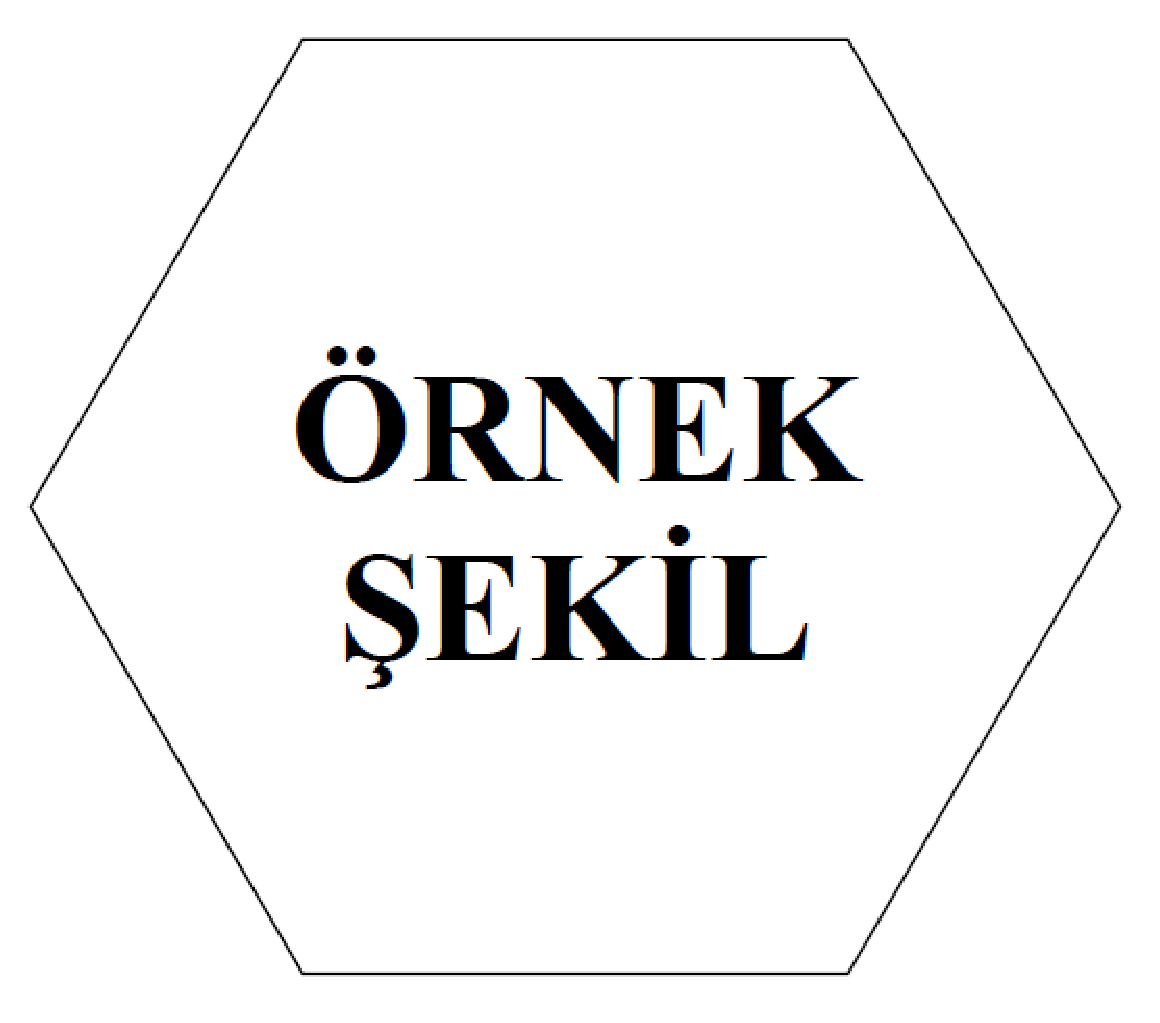
\includegraphics[width=230pt,keepaspectratio=true]{./fig/sekil6}
	% sekil6.eps: 0x0 pixel, 300dpi, 0.00x0.00 cm, bb=14 14 555 489
	\caption{Example figure.}
	\label{Figure4.1}
\end{figure}

This indicates that the ANN is accurate at base flow and flow height values lower then 3 m. 

\begin{table*}[h]
	{\setlength{\tabcolsep}{14pt}
		\caption{Example table.}
		\begin{center}
			\vspace{-6mm}
			\begin{tabular}{cccc}
				\hline \\[-2.45ex] \hline \\[-2.1ex]
				Column A & Column B & Column C & Column D \\
				\hline \\[-1.8ex]
				Row A & Row A & Row A & Row A \\
				Row B & Row B & Row B & Row B \\
				Row C & Row C & Row C & Row C \\
				[-0ex] \hline
			\end{tabular}
			\vspace{-6mm}
		\end{center}
		\label{Table4.1}}
\end{table*}

Stet clita kasd gub rgren, no sea takimata sanctus est Lorem ipsum dolor sit amet, consetetur sadipscing elitr, sed diam nonumy eirmod tempor invidunt ut lab ore sit et dolore magna. Stet clita kasd gub rgren, no sea takimata sanctus est Lorem ipsum dolor sit amet, consetetur sadipscing elitr, sed diam nonumy eirmod tempor invidunt ut lab ore sit et dolore magna.

Stet clita kasd gub rgren, no sea takimata sanctus est Lorem ipsum dolor sit amet, consetetur sadipscing elitr, sed diam nonumy eirmod tempor invidunt ut lab ore sit et dolore magna.  